\documentclass{ximera}

%\usepackage{todonotes}

\newcommand{\todo}{}

\usepackage{esint} % for \oiint
\ifxake%%https://math.meta.stackexchange.com/questions/9973/how-do-you-render-a-closed-surface-double-integral
\renewcommand{\oiint}{{\large\bigcirc}\kern-1.56em\iint}
\fi


\graphicspath{
  {./}
  {ximeraTutorial/}
  {basicPhilosophy/}
  {functionsOfSeveralVariables/}
  {normalVectors/}
  {lagrangeMultipliers/}
  {vectorFields/}
  {greensTheorem/}
  {shapeOfThingsToCome/}
  {dotProducts/}
  {partialDerivativesAndTheGradientVector/}
  {../productAndQuotientRules/exercises/}
  {../normalVectors/exercisesParametricPlots/}
  {../continuityOfFunctionsOfSeveralVariables/exercises/}
  {../partialDerivativesAndTheGradientVector/exercises/}
  {../directionalDerivativeAndChainRule/exercises/}
  {../commonCoordinates/exercisesCylindricalCoordinates/}
  {../commonCoordinates/exercisesSphericalCoordinates/}
  {../greensTheorem/exercisesCurlAndLineIntegrals/}
  {../greensTheorem/exercisesDivergenceAndLineIntegrals/}
  {../shapeOfThingsToCome/exercisesDivergenceTheorem/}
  {../greensTheorem/}
  {../shapeOfThingsToCome/}
  {../separableDifferentialEquations/exercises/}
  {vectorFields/}
}

\newcommand{\mooculus}{\textsf{\textbf{MOOC}\textnormal{\textsf{ULUS}}}}

\usepackage{tkz-euclide}
\usepackage{tikz}
\usepackage{tikz-cd}
\usetikzlibrary{arrows}
\tikzset{>=stealth,commutative diagrams/.cd,
  arrow style=tikz,diagrams={>=stealth}} %% cool arrow head
\tikzset{shorten <>/.style={ shorten >=#1, shorten <=#1 } } %% allows shorter vectors

\usetikzlibrary{backgrounds} %% for boxes around graphs
\usetikzlibrary{shapes,positioning}  %% Clouds and stars
\usetikzlibrary{matrix} %% for matrix
\usepgfplotslibrary{polar} %% for polar plots
\usepgfplotslibrary{fillbetween} %% to shade area between curves in TikZ
%\usetkzobj{all}
\usepackage[makeroom]{cancel} %% for strike outs
%\usepackage{mathtools} %% for pretty underbrace % Breaks Ximera
%\usepackage{multicol}
\usepackage{pgffor} %% required for integral for loops



%% http://tex.stackexchange.com/questions/66490/drawing-a-tikz-arc-specifying-the-center
%% Draws beach ball
\tikzset{pics/carc/.style args={#1:#2:#3}{code={\draw[pic actions] (#1:#3) arc(#1:#2:#3);}}}



\usepackage{array}
\setlength{\extrarowheight}{+.1cm}
\newdimen\digitwidth
\settowidth\digitwidth{9}
\def\divrule#1#2{
\noalign{\moveright#1\digitwidth
\vbox{\hrule width#2\digitwidth}}}




% \newcommand{\RR}{\mathbb R}
% \newcommand{\R}{\mathbb R}
% \newcommand{\N}{\mathbb N}
% \newcommand{\Z}{\mathbb Z}

\newcommand{\sagemath}{\textsf{SageMath}}


%\renewcommand{\d}{\,d\!}
%\renewcommand{\d}{\mathop{}\!d}
%\newcommand{\dd}[2][]{\frac{\d #1}{\d #2}}
%\newcommand{\pp}[2][]{\frac{\partial #1}{\partial #2}}
% \renewcommand{\l}{\ell}
%\newcommand{\ddx}{\frac{d}{\d x}}

% \newcommand{\zeroOverZero}{\ensuremath{\boldsymbol{\tfrac{0}{0}}}}
%\newcommand{\inftyOverInfty}{\ensuremath{\boldsymbol{\tfrac{\infty}{\infty}}}}
%\newcommand{\zeroOverInfty}{\ensuremath{\boldsymbol{\tfrac{0}{\infty}}}}
%\newcommand{\zeroTimesInfty}{\ensuremath{\small\boldsymbol{0\cdot \infty}}}
%\newcommand{\inftyMinusInfty}{\ensuremath{\small\boldsymbol{\infty - \infty}}}
%\newcommand{\oneToInfty}{\ensuremath{\boldsymbol{1^\infty}}}
%\newcommand{\zeroToZero}{\ensuremath{\boldsymbol{0^0}}}
%\newcommand{\inftyToZero}{\ensuremath{\boldsymbol{\infty^0}}}



% \newcommand{\numOverZero}{\ensuremath{\boldsymbol{\tfrac{\#}{0}}}}
% \newcommand{\dfn}{\textbf}
% \newcommand{\unit}{\,\mathrm}
% \newcommand{\unit}{\mathop{}\!\mathrm}
% \newcommand{\eval}[1]{\bigg[ #1 \bigg]}
% \newcommand{\seq}[1]{\left( #1 \right)}
% \renewcommand{\epsilon}{\varepsilon}
% \renewcommand{\phi}{\varphi}


% \renewcommand{\iff}{\Leftrightarrow}

% \DeclareMathOperator{\arccot}{arccot}
% \DeclareMathOperator{\arcsec}{arcsec}
% \DeclareMathOperator{\arccsc}{arccsc}
% \DeclareMathOperator{\si}{Si}
% \DeclareMathOperator{\scal}{scal}
% \DeclareMathOperator{\sign}{sign}


%% \newcommand{\tightoverset}[2]{% for arrow vec
%%   \mathop{#2}\limits^{\vbox to -.5ex{\kern-0.75ex\hbox{$#1$}\vss}}}
% \newcommand{\arrowvec}[1]{{\overset{\rightharpoonup}{#1}}}
% \renewcommand{\vec}[1]{\arrowvec{\mathbf{#1}}}
% \renewcommand{\vec}[1]{{\overset{\boldsymbol{\rightharpoonup}}{\mathbf{#1}}}}

% \newcommand{\point}[1]{\left(#1\right)} %this allows \vector{ to be changed to \vector{ with a quick find and replace
% \newcommand{\pt}[1]{\mathbf{#1}} %this allows \vec{ to be changed to \vec{ with a quick find and replace
% \newcommand{\Lim}[2]{\lim_{\point{#1} \to \point{#2}}} %Bart, I changed this to point since I want to use it.  It runs through both of the exercise and exerciseE files in limits section, which is why it was in each document to start with.

% \DeclareMathOperator{\proj}{\mathbf{proj}}
% \newcommand{\veci}{{\boldsymbol{\hat{\imath}}}}
% \newcommand{\vecj}{{\boldsymbol{\hat{\jmath}}}}
% \newcommand{\veck}{{\boldsymbol{\hat{k}}}}
% \newcommand{\vecl}{\vec{\boldsymbol{\l}}}
% \newcommand{\uvec}[1]{\mathbf{\hat{#1}}}
% \newcommand{\utan}{\mathbf{\hat{t}}}
% \newcommand{\unormal}{\mathbf{\hat{n}}}
% \newcommand{\ubinormal}{\mathbf{\hat{b}}}

% \newcommand{\dotp}{\bullet}
% \newcommand{\cross}{\boldsymbol\times}
% \newcommand{\grad}{\boldsymbol\nabla}
% \newcommand{\divergence}{\grad\dotp}
% \newcommand{\curl}{\grad\cross}
%\DeclareMathOperator{\divergence}{divergence}
%\DeclareMathOperator{\curl}[1]{\grad\cross #1}
% \newcommand{\lto}{\mathop{\longrightarrow\,}\limits}

% \renewcommand{\bar}{\overline}

\colorlet{textColor}{black}
\colorlet{background}{white}
\colorlet{penColor}{blue!50!black} % Color of a curve in a plot
\colorlet{penColor2}{red!50!black}% Color of a curve in a plot
\colorlet{penColor3}{red!50!blue} % Color of a curve in a plot
\colorlet{penColor4}{green!50!black} % Color of a curve in a plot
\colorlet{penColor5}{orange!80!black} % Color of a curve in a plot
\colorlet{penColor6}{yellow!70!black} % Color of a curve in a plot
\colorlet{fill1}{penColor!20} % Color of fill in a plot
\colorlet{fill2}{penColor2!20} % Color of fill in a plot
\colorlet{fillp}{fill1} % Color of positive area
\colorlet{filln}{penColor2!20} % Color of negative area
\colorlet{fill3}{penColor3!20} % Fill
\colorlet{fill4}{penColor4!20} % Fill
\colorlet{fill5}{penColor5!20} % Fill
\colorlet{gridColor}{gray!50} % Color of grid in a plot

\newcommand{\surfaceColor}{violet}
\newcommand{\surfaceColorTwo}{redyellow}
\newcommand{\sliceColor}{greenyellow}




\pgfmathdeclarefunction{gauss}{2}{% gives gaussian
  \pgfmathparse{1/(#2*sqrt(2*pi))*exp(-((x-#1)^2)/(2*#2^2))}%
}


%%%%%%%%%%%%%
%% Vectors
%%%%%%%%%%%%%

%% Simple horiz vectors
\renewcommand{\vector}[1]{\left\langle #1\right\rangle}


%% %% Complex Horiz Vectors with angle brackets
%% \makeatletter
%% \renewcommand{\vector}[2][ , ]{\left\langle%
%%   \def\nextitem{\def\nextitem{#1}}%
%%   \@for \el:=#2\do{\nextitem\el}\right\rangle%
%% }
%% \makeatother

%% %% Vertical Vectors
%% \def\vector#1{\begin{bmatrix}\vecListA#1,,\end{bmatrix}}
%% \def\vecListA#1,{\if,#1,\else #1\cr \expandafter \vecListA \fi}

%%%%%%%%%%%%%
%% End of vectors
%%%%%%%%%%%%%

%\newcommand{\fullwidth}{}
%\newcommand{\normalwidth}{}



%% makes a snazzy t-chart for evaluating functions
%\newenvironment{tchart}{\rowcolors{2}{}{background!90!textColor}\array}{\endarray}

%%This is to help with formatting on future title pages.
\newenvironment{sectionOutcomes}{}{}



%% Flowchart stuff
%\tikzstyle{startstop} = [rectangle, rounded corners, minimum width=3cm, minimum height=1cm,text centered, draw=black]
%\tikzstyle{question} = [rectangle, minimum width=3cm, minimum height=1cm, text centered, draw=black]
%\tikzstyle{decision} = [trapezium, trapezium left angle=70, trapezium right angle=110, minimum width=3cm, minimum height=1cm, text centered, draw=black]
%\tikzstyle{question} = [rectangle, rounded corners, minimum width=3cm, minimum height=1cm,text centered, draw=black]
%\tikzstyle{process} = [rectangle, minimum width=3cm, minimum height=1cm, text centered, draw=black]
%\tikzstyle{decision} = [trapezium, trapezium left angle=70, trapezium right angle=110, minimum width=3cm, minimum height=1cm, text centered, draw=black]


\title{Function of Change}

\begin{document}

\begin{abstract}
rate as a relationship
\end{abstract}
\maketitle






\section{Rate of Change Over an Interval}





Consider the function $Q(x) = \frac{(x+7)(x-5)}{5}$








\begin{image}
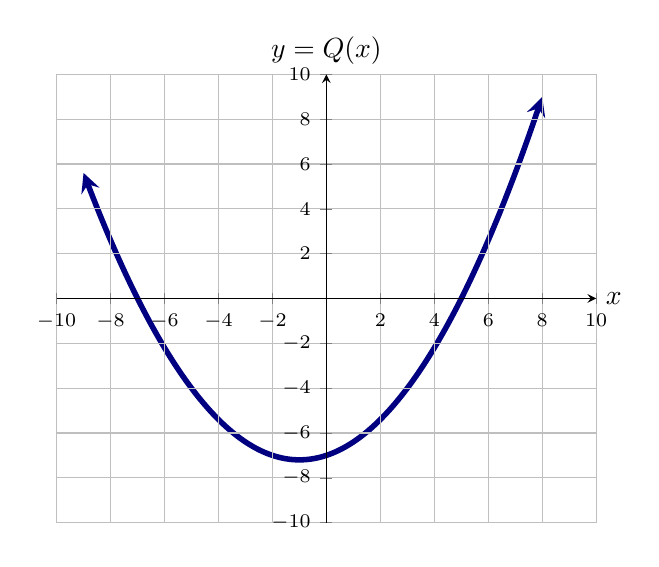
\begin{tikzpicture}
  \begin{axis}[
            domain=-10:10, ymax=10, xmax=10, ymin=-10, xmin=-10,
            axis lines =center, xlabel=$x$, ylabel={$y=Q(x)$}, grid = major,
            ytick={-10,-8,-6,-4,-2,2,4,6,8,10},
            xtick={-10,-8,-6,-4,-2,2,4,6,8,10},
            yticklabels={$-10$,$-8$,$-6$,$-4$,$-2$,$2$,$4$,$6$,$8$,$10$}, 
            xticklabels={$-10$,$-8$,$-6$,$-4$,$-2$,$2$,$4$,$6$,$8$,$10$},
            ticklabel style={font=\scriptsize},
            every axis y label/.style={at=(current axis.above origin),anchor=south},
            every axis x label/.style={at=(current axis.right of origin),anchor=west},
            axis on top
          ]
          
          %\addplot [line width=2, penColor2, smooth,samples=100,domain=(-6:2)] {-2*x-3};
            \addplot [line width=2, penColor, smooth,samples=100,domain=(-9:8),<->] {.2*(x+7)*(x-5)};

          %\addplot[color=penColor,fill=penColor2,only marks,mark=*] coordinates{(-6,9)};
          %\addplot[color=penColor,fill=penColor2,only marks,mark=*] coordinates{(2,-7)};



           

  \end{axis}
\end{tikzpicture}
\end{image}




The rate-of-change over the interval $[-3, 4]$ is 
\[  \frac{Q(4)-Q(-3)}{4-(-3)} = \frac{4.2}{7} = 0.6      \]


This is the slope of the secant line through the points $(-3, Q(-3))$ and $(4, Q(4))$.











\begin{image}
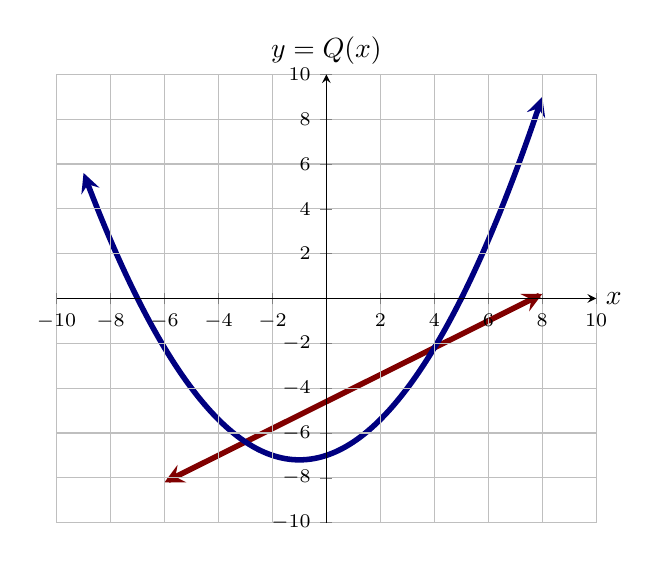
\begin{tikzpicture}
  \begin{axis}[
            domain=-10:10, ymax=10, xmax=10, ymin=-10, xmin=-10,
            axis lines =center, xlabel=$x$, ylabel={$y=Q(x)$}, grid = major,
            ytick={-10,-8,-6,-4,-2,2,4,6,8,10},
            xtick={-10,-8,-6,-4,-2,2,4,6,8,10},
            yticklabels={$-10$,$-8$,$-6$,$-4$,$-2$,$2$,$4$,$6$,$8$,$10$}, 
            xticklabels={$-10$,$-8$,$-6$,$-4$,$-2$,$2$,$4$,$6$,$8$,$10$},
            ticklabel style={font=\scriptsize},
            every axis y label/.style={at=(current axis.above origin),anchor=south},
            every axis x label/.style={at=(current axis.right of origin),anchor=west},
            axis on top
          ]
          
            \addplot [line width=2, penColor2, smooth,samples=100,domain=(-6:8),<->] {0.6*(x+3)-6.4};
            \addplot [line width=2, penColor, smooth,samples=100,domain=(-9:8),<->] {.2*(x+7)*(x-5)};

          %\addplot[color=penColor,fill=penColor2,only marks,mark=*] coordinates{(-6,9)};
          %\addplot[color=penColor,fill=penColor2,only marks,mark=*] coordinates{(2,-7)};



           

  \end{axis}
\end{tikzpicture}
\end{image}




This rate-of-change is the \textbf{constant} rate-of-change that would be needed in order for a linear funciton to match the endpoint values of the function.  Of course, we can see from the graph that this rate-of-change varies depending on the interval selected. 

$[-3, 4]$ would not be a good interval to use if you were interested in the rate-of-change near $-3$.

$[-3, -2.5]$ would probably give a better interval. 






The rate-of-change over the interval $[-3, -2.5]$ is 
\[  \frac{Q(-2.5)-Q(-3)}{-2.5-(-3)} = \frac{-0.35}{0.5} = -0.7      \]


This is the slope of the secant line through the points $(-3, Q(-3))$ and $(-2.5, Q(-2.5))$.











\begin{image}
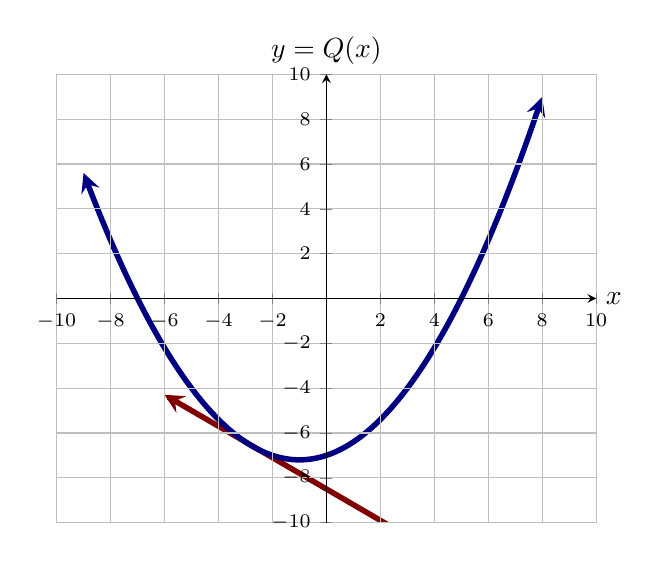
\begin{tikzpicture}
  \begin{axis}[
            domain=-10:10, ymax=10, xmax=10, ymin=-10, xmin=-10,
            axis lines =center, xlabel=$x$, ylabel={$y=Q(x)$}, grid = major,
            ytick={-10,-8,-6,-4,-2,2,4,6,8,10},
            xtick={-10,-8,-6,-4,-2,2,4,6,8,10},
            yticklabels={$-10$,$-8$,$-6$,$-4$,$-2$,$2$,$4$,$6$,$8$,$10$}, 
            xticklabels={$-10$,$-8$,$-6$,$-4$,$-2$,$2$,$4$,$6$,$8$,$10$},
            ticklabel style={font=\scriptsize},
            every axis y label/.style={at=(current axis.above origin),anchor=south},
            every axis x label/.style={at=(current axis.right of origin),anchor=west},
            axis on top
          ]
          
            \addplot [line width=2, penColor2, smooth,samples=100,domain=(-6:8),<->] {-0.7*(x+3)-6.4};
            \addplot [line width=2, penColor, smooth,samples=100,domain=(-9:8),<->] {.2*(x+7)*(x-5)};

          %\addplot[color=penColor,fill=penColor2,only marks,mark=*] coordinates{(-6,9)};
          %\addplot[color=penColor,fill=penColor2,only marks,mark=*] coordinates{(2,-7)};



           

  \end{axis}
\end{tikzpicture}
\end{image}




That is looking more like a tangent line, than a secant.





\begin{idea}
\textbf{\textcolor{green!50!black}{Tangent Line}}

A tangent line to a graph at a point, is first a line. Second it intersects the graph at a given point, called the \textbf{point of tangency} or the \textbf{tangent point}. Third, it does the best job of pretending to be the graph \textbf{\textcolor{red!70!darkgray}{at that point}}. \\




The tangent point below is $\left( -3, -\frac{32}{5} \right)$. If you zoom in on the intersection point (a lot), then the parabola will slowly appear to become a line. The tangent line is the line the graph is becoming. 






\begin{center}
\desmos{rufcna7r3b}{400}{300}
\end{center}



It is like the tangent line and the graph have the same slope at the tangent point.

\end{idea}










\section*{Rate of Change Over a Single Number?}





If we make a really small interval at $-3$, then the slope of the secant line should give a good approximation of the tangent line.  The slope of the secant line should approximate the slope of the tangent line.




The rate-of-change over the interval $[-3, -3+h]$ is 
\[  \frac{Q(-3+h)-Q(-3)}{(-3+h)-(-3)} = \frac{Q(-3+h)-Q(-3)}{h} =  \frac{\frac{(-3+h+7)(-3+h-5)}{5}+64}{h}   \]


This is the slope of the secant line through the points $(-3, Q(-3))$ and $(-3+h, Q(-3+h))$, which is very near the tangent line at $(-3, Q(-3))$, when $h$ is small.



By moving the value of $h$ close to $0$, we can get a good estimate of the slope of the tangent line.









\begin{center}
\desmos{di7qdhdfnn}{400}{300}
\end{center}




The slope of the line tangent to the graph at $(-3, -6.4)$ looks to be about $-0.8$.

Of course $-3$ was nothing special.  We can get slopes of tangent lines at any point on the graph. Let's move around the graph and record the tangent line slopes.  We'll record visually.

The slope of the tangent line at $-3$ is $-0.8$, so we'll plot the point $(-3,-0.8)$ to record this information.  This will be a visual encoding of the tangent slope for the domain number $-3$.





\begin{image}
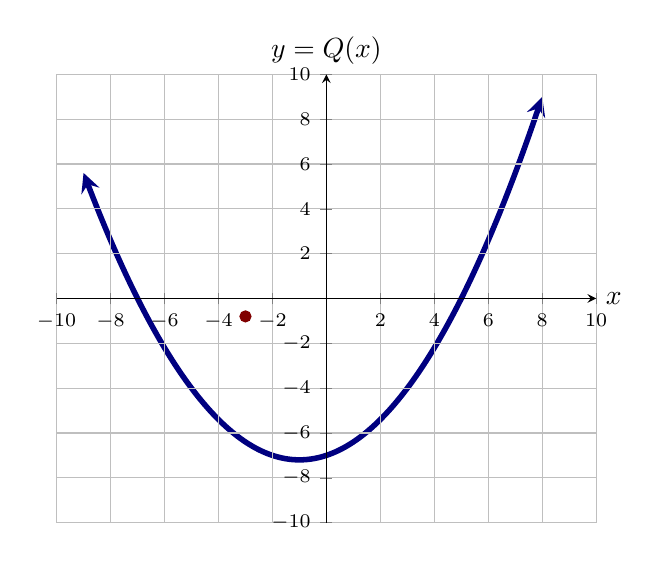
\begin{tikzpicture}
  \begin{axis}[
            domain=-10:10, ymax=10, xmax=10, ymin=-10, xmin=-10,
            axis lines =center, xlabel=$x$, ylabel={$y=Q(x)$}, grid = major,
            ytick={-10,-8,-6,-4,-2,2,4,6,8,10},
            xtick={-10,-8,-6,-4,-2,2,4,6,8,10},
            yticklabels={$-10$,$-8$,$-6$,$-4$,$-2$,$2$,$4$,$6$,$8$,$10$}, 
            xticklabels={$-10$,$-8$,$-6$,$-4$,$-2$,$2$,$4$,$6$,$8$,$10$},
            ticklabel style={font=\scriptsize},
            every axis y label/.style={at=(current axis.above origin),anchor=south},
            every axis x label/.style={at=(current axis.right of origin),anchor=west},
            axis on top
          ]
          
            %\addplot [line width=2, penColor2, smooth,samples=100,domain=(-6:8),<->] {-0.7*(x+3)-6.4};
            \addplot [line width=2, penColor, smooth,samples=100,domain=(-9:8),<->] {.2*(x+7)*(x-5)};

          	\addplot[color=penColor2,fill=penColor2,only marks,mark=*] coordinates{(-3,-0.8)};




           

  \end{axis}
\end{tikzpicture}
\end{image}


We could do this for a bunch of domain numbers.

\begin{enumerate}
\item select a domain number
\item select a very tiny interval beginning at that domain number
\item calculate the rate-of-change over the tiny interval
\item plot a point on the graph.  First coordinate is the domain number.  Second coordinate is the rate-of-change.
\end{enumerate}







\begin{image}
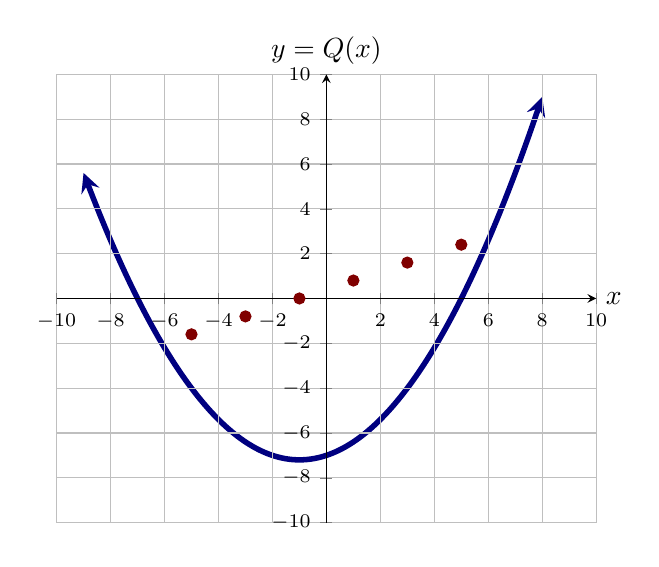
\begin{tikzpicture}
  \begin{axis}[
            domain=-10:10, ymax=10, xmax=10, ymin=-10, xmin=-10,
            axis lines =center, xlabel=$x$, ylabel={$y=Q(x)$}, grid = major,
            ytick={-10,-8,-6,-4,-2,2,4,6,8,10},
            xtick={-10,-8,-6,-4,-2,2,4,6,8,10},
            yticklabels={$-10$,$-8$,$-6$,$-4$,$-2$,$2$,$4$,$6$,$8$,$10$}, 
            xticklabels={$-10$,$-8$,$-6$,$-4$,$-2$,$2$,$4$,$6$,$8$,$10$},
            ticklabel style={font=\scriptsize},
            every axis y label/.style={at=(current axis.above origin),anchor=south},
            every axis x label/.style={at=(current axis.right of origin),anchor=west},
            axis on top
          ]
          
            %\addplot [line width=2, penColor2, smooth,samples=100,domain=(-6:8),<->] {-0.7*(x+3)-6.4};
            \addplot [line width=2, penColor, smooth,samples=100,domain=(-9:8),<->] {.2*(x+7)*(x-5)};

          	\addplot[color=penColor2,fill=penColor2,only marks,mark=*] coordinates{(-5,-1.6)};
          	\addplot[color=penColor2,fill=penColor2,only marks,mark=*] coordinates{(-3,-0.8)};
          	\addplot[color=penColor2,fill=penColor2,only marks,mark=*] coordinates{(-1,0)};
          	\addplot[color=penColor2,fill=penColor2,only marks,mark=*] coordinates{(1,0.8)};
          	\addplot[color=penColor2,fill=penColor2,only marks,mark=*] coordinates{(3,1.6)};
          	\addplot[color=penColor2,fill=penColor2,only marks,mark=*] coordinates{(5,2.4)};




           

  \end{axis}
\end{tikzpicture}
\end{image}






If we do this for every domain number, then we will have created a new function.  Every domain number will be paired with the slope of the tangent line at the corresponding point.

We could graph this ``slope function''.







\begin{center}
\desmos{xv5dnwhbku}{400}{300}
\end{center}




This function, whose values are the rates-of-change of another function, is called the \textbf{derivative} of the other function, because it was derived from the original function.




$\blacktriangleright$ Let $f$ be a function.  Then the derivative of $f$ is denoted as $f'$. People pronounce this as ``\textit{f prime}''. \\



\begin{definition} \textbf{\textcolor{green!50!black}{The Derivative - The Slope Function}} 

Let $f$ be a function.

Then $f'$ represents the \textbf{derivative of $f$}.


$f'(a) = $ the slope of the tangent line at $(a, f(a))$, on the graph of $f$.




\end{definition}



Through the slope of the tangent line, we have invented a way of talking about the \textbf{\textcolor{purple!85!blue}{instantaneous rate of change}} of a function at a number, rather than over an interval. \\









\begin{example}



The function $Q(x) = \frac{(x+7)(x-5)}{5}$ is a quadratic and has a parabola for a graph.  The vertex, $(-1, \tfrac{-36}{5})$, of the parabola has a horizontal tangent line, $y=\tfrac{-36}{5}$.











\begin{image}
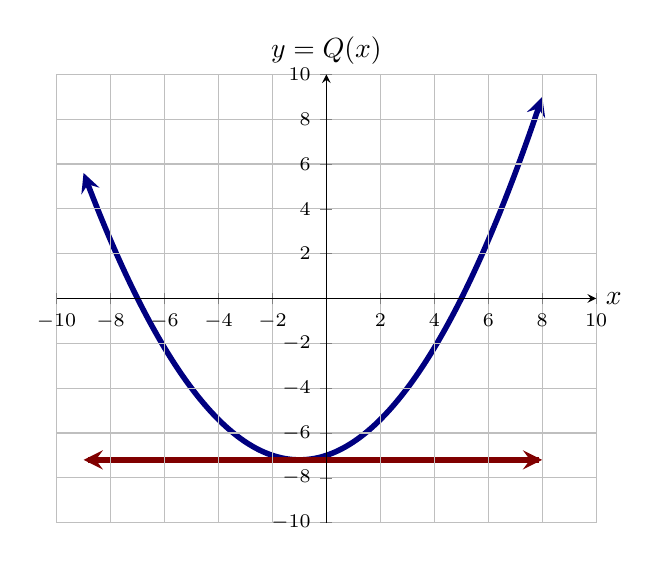
\begin{tikzpicture}
  \begin{axis}[
            domain=-10:10, ymax=10, xmax=10, ymin=-10, xmin=-10,
            axis lines =center, xlabel=$x$, ylabel={$y=Q(x)$}, grid = major,
            ytick={-10,-8,-6,-4,-2,2,4,6,8,10},
            xtick={-10,-8,-6,-4,-2,2,4,6,8,10},
            yticklabels={$-10$,$-8$,$-6$,$-4$,$-2$,$2$,$4$,$6$,$8$,$10$}, 
            xticklabels={$-10$,$-8$,$-6$,$-4$,$-2$,$2$,$4$,$6$,$8$,$10$},
            ticklabel style={font=\scriptsize},
            every axis y label/.style={at=(current axis.above origin),anchor=south},
            every axis x label/.style={at=(current axis.right of origin),anchor=west},
            axis on top
          ]
          
            %\addplot [line width=2, penColor2, smooth,samples=100,domain=(-6:8),<->] {-0.7*(x+3)-6.4};
            \addplot [line width=2, penColor, smooth,samples=100,domain=(-9:8),<->] {.2*(x+7)*(x-5)};

            \addplot [line width=2, penColor2, smooth,samples=100,domain=(-9:8),<->] {-7.2};

           

  \end{axis}
\end{tikzpicture}
\end{image}



The slope of this tangent line is $0$.  Therefore, $Q'(-1) = 0$.



\end{example}





















\begin{example} The Derivative





Graph of $y = f(x) = e^{\tfrac{x}{5}}$







\begin{image}
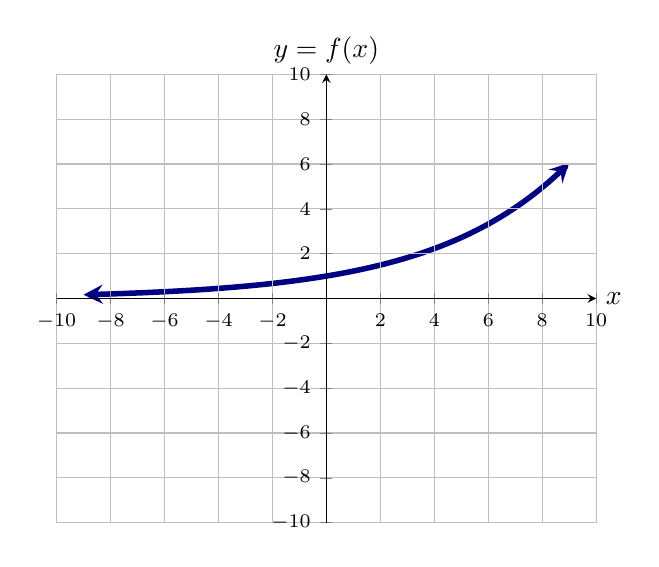
\begin{tikzpicture}
  \begin{axis}[
            domain=-10:10, ymax=10, xmax=10, ymin=-10, xmin=-10,
            axis lines =center, xlabel=$x$, ylabel={$y=f(x)$}, grid = major,
            ytick={-10,-8,-6,-4,-2,2,4,6,8,10},
            xtick={-10,-8,-6,-4,-2,2,4,6,8,10},
            yticklabels={$-10$,$-8$,$-6$,$-4$,$-2$,$2$,$4$,$6$,$8$,$10$}, 
            xticklabels={$-10$,$-8$,$-6$,$-4$,$-2$,$2$,$4$,$6$,$8$,$10$},
            ticklabel style={font=\scriptsize},
            every axis y label/.style={at=(current axis.above origin),anchor=south},
            every axis x label/.style={at=(current axis.right of origin),anchor=west},
            axis on top
          ]
          
            %\addplot [line width=2, penColor2, smooth,samples=100,domain=(-6:8),<->] {-0.7*(x+3)-6.4};
            \addplot [line width=2, penColor, smooth,samples=100,domain=(-9:9),<->] {e^(0.2*x)};


           

  \end{axis}
\end{tikzpicture}
\end{image}




The value of $f'(4)$ is
\begin{multipleChoice}
\choice[correct]{positive}
\choice{negative}
\end{multipleChoice}





\end{example}










\begin{example}



Here is a graph of $y = g(x) = \sin(x)$ and $g'(x)$.






\begin{center}
\desmos{yp5zobfigx}{400}{300}
\end{center}



The derivative of $\sin(x)$ is
\begin{multipleChoice}
\choice[correct]{$\cos(x)$}
\choice{$\sin(x)$}
\choice{$-\cos(x)$}
\choice{$-\sin(x)$}
\end{multipleChoice}


\end{example}
































\begin{center}
\textbf{\textcolor{green!50!black}{ooooo-=-=-=-ooOoo-=-=-=-ooooo}} \\

more examples can be found by following this link\\ \link[More Examples of Rate of Change]{https://ximera.osu.edu/csccmathematics/precalculus1/precalculus1/rateOfChange/examples/exampleList}

\end{center}















\end{document}